\begin{figure}[htbp]
\centering
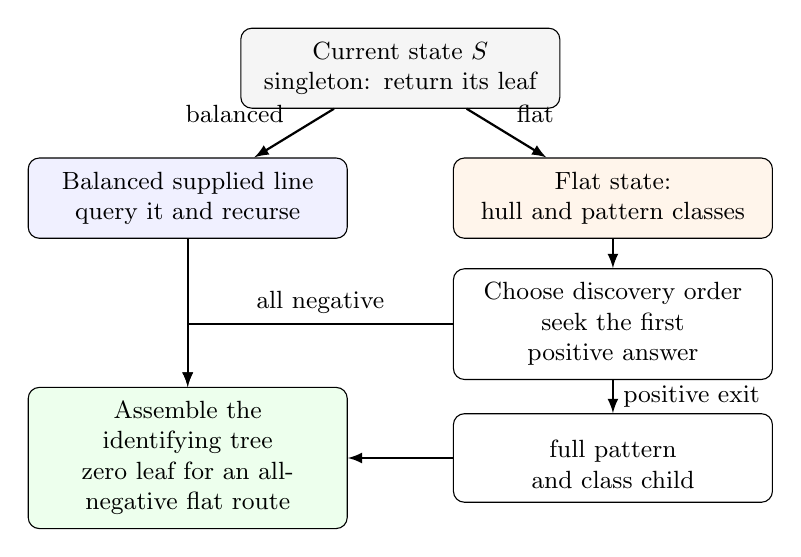
\begin{tikzpicture}[every node/.style={font=\small},
  box/.style={draw,rounded corners,align=center,inner sep=5pt,text width=3.7cm},
  arr/.style={-latex,thick}]
  \node[box,fill=gray!8] (state) at (0,0) {Current state $S$\\singleton: return its leaf};
  \node[box,fill=blue!6] (balanced) at (-2.7,-1.65)
    {Balanced supplied line\\query it and recurse};
  \node[box,fill=orange!8] (flat) at (2.7,-1.65)
    {Flat state: \HullData\\hull and pattern classes};
  \node[box] (discover) at (2.7,-3.25)
    {Choose discovery order\\seek the first positive answer};
  \node[box] (decode) at (2.7,-4.95)
    {\EndpointCode\\full pattern and class child};
  \node[box,fill=green!7] (output) at (-2.7,-4.95)
    {Assemble the identifying tree\\zero leaf for an all-negative flat route};
  \draw[arr] (state) -- node[above left]{balanced} (balanced);
  \draw[arr] (state) -- node[above right]{flat} (flat);
  \draw[arr] (flat) -- (discover);
  \draw[arr] (discover) -- node[right]{positive exit} (decode);
  \draw[arr] (discover.west) -- node[above]{all negative} (-2.7,-3.25)
    -- (output.north);
  \draw[arr] (decode) -- (output);
  \draw[arr] (balanced) -- (output);
\end{tikzpicture}
\caption{The common recursive structure. Arrows describe the output of
one stage passed to the next. The maximum-depth routines construct class
children before choosing the schedule, so their stored heights can set
deadlines; expected-depth routines use original prior masses. The flat
stage has an all-negative leaf only when the zero pattern is present.
Scheduling and decoding use supplied hull lines.}
\label{fig:recursive-procedure-flow}
\end{figure}

